%!TeX program = xelatex
%!TeX builder = latexmk
\documentclass{mcmthesis}
\usepackage{bigstrut}
\usepackage{graphicx}

\usepackage[caption=false,font=footnotesize]{subfig}
\usepackage{caption}
%\usepackage{subfigure}
\usepackage[ruled]{algorithm}
\usepackage{algorithmic}
\mcmsetup{tcn = 1921597, problem = D, titlepage = false, titleinsheet = false}
%\usepackage{indentfirst}
%\setlength{\parindent}{2em}

\usepackage{blindtext}      % 提供 \blindtext 命令,演示用
\title{Safe Evacuation Taking No Time}
\author{Li Xinrui}
\date{today}
\usepackage{fontspec}
%\newfontfamily\monaco{Monaco}

\usepackage{listings, lstautogobble}
\lstset{
	numbers=left,
	%numberstyle=\tiny\monaco,
	%basicstyle=\small\monaco,
	autogobble=true
}
\begin{document}
	
	\begin{abstract}
		
		
		The world has witnessed the rise of terrorist attacks since the 21st century. Terrorists have stretched their claws from hazardous to peaceful regions, especially Europe. The incident of terror attacks in the Louvre arouses our reconsideration of emergency evacuation plans of famous sites. Modeling emergency evacuation plans, which is crucial to tackling the problem, is an intricate issue concerning the capacity of the flow and clearance time of evacuation. In this article we construct two models, the first model is a game theory based  individual behavior simulation model. After evaluation, we come up with vacuation time optimization model using network analysis methodology. After that, we revise the previous model by introducing parallel edges and bidirectional flow control  to figure out an efficient evacuation plan.
		
		In the first place, the game theory based model is established to calculate the optimum evacuation plans for all the evacuees individually. The model will simulate the situation where everyone chooses evacuation routes with a selfish strategy, which will achieve the Nash equilibrium after iterations. Nevertheless, the nature of homogeneity of evacuees in this model limits the model’s explanatory scope. Hence, we adjust our presumptions and revise our model. 
		
		Next, we change our perspective to treat evacuees as a flow, and set up an optimized evacuation time model based on network analysis. This model is capable of coordinate people's choices for the optimal evacuation time given the safe population density. By collecting and calculating the statistics collected from Google map, we figure out the optimal evacuation time is 647s based on an average flow. 
		
		Then we go on modifying the model to unravel the optimization evacuation time under restrictions. For the disabled and the elder, we introduce parallel edges. We divide an edge into two parts, one of which has a lower travel speed.  In this way, our model can simulate the situation when the disabled and the elder are involved in the evacuation.
		
		For the emergency personnel, we introduce reversed edges and bidirectional flow control to defuse the convection problem. The reversed edges share the capacity with the original edge, the flow control is realized by adding virtual nodes and virtual edges. By this modification, our model can analyze the optimal evacuation time with emergency personnel entering the building.
		
		Finally, we testify our model's sensibility and scalability. When  potential threats block out segments of the evacuation path, the model remains reliable. As for scalability, we proved it by algorithm analysis and numerical experiment.
		
		
	\end{abstract}
	
	\maketitle                  % 打印控制页等
	
	\tableofcontents
	\newpage
	
	\section{Introduction}
	\subsection{Background}
	
	The menace posed by terrorists has skyrocketed over the past decade, especially with the rise of ISIS.  The number of terrorist incidents has increased since 2010, along with the number of fatalities, both reaching peaks in 2014. That year, the world suffered from 16903 terrorist attacks and 44490 deaths.(our world in data) Amongst regions attacked by terrorism, Europe has been facing the greatest challenges, in which France is the critical target. From the major terrorist attack in Bataclan concert hall in November 2015 to Christmas market attack in Strasbourg in 2018, France has witnessed a dramatic increase in terrorist activities since 2014.
	
	Normally, terrorists tend to launch attacks in tourist spots with large crowds. As one of the world's largest and most visited sites, the Lourve underwent a terrorist threat in 2017. During the attack, most visitors were instructed to stay still in the Lourve even after the perpetrator was caught.() It is obvious that the current emergency plans cannot solve the new arising terrorist issues. Hence, to evacuate the visitors quickly and safely, an adaptable evacuation plan necessitates a thorough reconsideration. 
	
	Meanwhile, an upgraded emergency plan should consider practical conditions and scrutinize any bottlenecks when it comes to implementation. While the emergency evacuation plan is tailored for the Lourve, it can still apply to other large and crowded mega-buildings which under potential threats with a little adjustment.
	
	
	\subsection{Our Work}
	Inspired by game theory, we design our own game theory model based on the shortest time for evacuation. Since individuals are rational, they may endeavor to leave the hazardous area as quickly as possible. In this model, we will calculate when evacuees’ behavioral reactions along with their movement and the capacity of all the routines reach a Nash equilibrium so that individual optimum strategy can be achieved and the shortest time evacuees use to leave the hazardous area can be unfolded. But this model has some limitations in terms of application scope, so we will introduce one more metric to solve the problem.
	
	After elaborating reasonable metrics on optimization models, we devise an evacuation time optimization model based on network flow. This model will give the answers of how can evacuees as a whole evacuate as fast as possible and how many time spent. 
	
	Additionally, we improve our evacuation time optimization model with some adjustment  so as to extend its applicability on diverse situations
	
	Lastly, we analyze the sensitivity and scalability of our models and discuss their merits and demerits.
	
	
	
	
	\section{Fundamental  Assumptions}
	We make the following assumptions about modeling process in this paper.
	\begin{enumerate}[1.]
		\item  Each evacuee is rational during the interactive decision-making process. That is to say, their behaviors will be based on the observed situation and logical reasoning and they will pursue solutions that meet their interest rationally.
		\item Evacuee will endeavor to leave the hazardous area as quickly as possible. We assume that  all the evacuees are selfish during an emergency so they need to compete with each other to gain the greatest chance to flee.
		\item The reaction time for the emergency and the fleeing time to egress sequence are neglected. Because both time mentioned above are short enough to overlook
		\item Visitors are assumed to flock in dense area with well-known displays. That is to say, evacuees start from the same node when emergency happens
		\item Evacuees will be under the command of emergency personnel. Based on the information provided by the problem, the majority visitors of the Lourve are visiting for the first time. So it is reasonable to assume that the visitors will follow the command of emergency personnel due to their low familiarity with the building.
		\item During emergency, the moving direction of all staircases will be altered towards emergency egress. In other words, evacuees have no difficulty in using staircases to leave the building.
		\item Once emergency emerges, all the closed exhibition rooms will be open. Emergency personnel of each floor are trained to react to emergency so they will open all the passageways to ensure free flow.
		\item There are no obstacles to evacuation in aisles.
	\end{enumerate}
	Given those preconditions, we can set out to construct our model so as to figure out a safe and efficient evacuation plan for the Louvre.
	
	\section{Notations and Descriptions}
	% Table generated by Excel2LaTeX from sheet 'Sheet1'
	\begin{tabular}{l|l}
		\hline
		$G(V,E)$  & A graph denoting the architectural structure of the Louvre
		\bigstrut\\
		\hline
		$V$  &  The set of vetex \bigstrut\\
		\hline
		$v_i$  & A node of $V$, represents a scenic spot, a corner in Louvre the  \bigstrut\\
		& or a crossing point of the passageway \\
		\hline
		$e_{i,j}​$  & The edge connecting two nodes $v_i$ and $v_j$, which can be a segment \\ 
		& of the corridor, a stair or an elevator \bigstrut\\
		\hline
		$​w_e$  & The width or the transport capacity of the  edge $e$  \bigstrut\\
		\hline
		$l_e$  & The length of the an edge $e$ \bigstrut\\
		\hline
		$R$  &  A route consisted of continuous edges  \bigstrut\\
		\hline
		$c_e$     & The cost of passing  an edge $e$ \bigstrut\\
		\hline
		$c_R$   & The sum of edge's cost on $R$  \bigstrut\\
		\hline
		$\rho_e$  &The density of the crowd  on an edge \bigstrut\\
		\hline
		$s_i$  & One of the source nodes in a network flow \bigstrut\\
		\hline
		$s_{super}​$  & The supersource, which is a virtual source connecting to all sources
		\bigstrut\\
		\hline
		$ex_i$     & One of the sink nodes in a network flow  \bigstrut\\
		\hline
		$ex_{super}$ &The supersink, which is a virtual source connected by all sinks 
		\bigstrut\\
		\hline
		$f_i$ & The instant flow of a arc \bigstrut\\
		\hline
		$F$ &  The accumulative flow of an arc over time \bigstrut\\
		\hline
		$vel$     &   People's walking speed in the Louvre \bigstrut\\
		\hline
	\end{tabular}%
	\label{tab:addlabel}%
	\section{The game theory based selfish evacuation  model}
	We construct game theory based individual behaviour simulation model to estimate the optimum strategy for evacuation in micro scope.
	
	
	\subsection{Theoretical Framework}
	In a complete information dynamic game, an individual will constantly change their options based on other’s decision, knowing the utility payoff and thus the choice of other players. 
	
	Within a game-theory-based scenario, a rational individual will choose the strategy that could maximize his/her utility payoff – in this case, everyone wants to escape this building as soon as possible, regardless of the overall evacuation time. In the simplest case, an individual will choose the closest exit in order to minimize escape time, but when the number of escapers is great enough, one must take into account the number of potential ‘rivals’ that will possibly choose the same exit, because other escapers could cause congestion and thus extra escape time. Since no one could forecast exactly how many people will choose the same exit as he/she chooses, the dynamic situation where all participants strive to find the best route for themselves on the basis of other’s choices is a game and the situation where everyone has no incentive to change his/her decision is a Nash Equilibrium.  
	
	
	In this model, we try to include both the consideration of distance to exit and the consideration of congestion as criteria to calculate utility payoff of each participant. After a dynamic adjustment process, an equilibrium is achieved. Finally, we can make simulations basing on everyone's decision to figure out the exact escape time.
	
	\subsection{Model Analysis}
	\subsubsection{Representation of The Louvre}
	
	We use an undirected graph $G(V,E)$ to model the architectural structure of Louvre. Each node $v_i \in V$ represents a scenic spot, a corner in Louvre the or a crossing point of the passageway. The edge $e_{i,j}$ connects node $v_i$ and $v_j$ means the segment of passageway connecting the two points in the Louvre, which can be a segment of the corridor, a stair or an elevator. We measure the width $w$ and length $l$ of the corridors and stairs $e_{i,j}$ using Google map. We also estimate the capacity of elevators by consulting \cite{xu2009staircase} and set the equivalent $w = 10, l = 30$.  Figure \ref{fig:subfig_gd} shows the ichnography of the ground floor and its corresponding graph representation. The number on the edge denotes the length.
	
	\begin{figure} 
		\centering 
		\subfloat[Ichnography]{ 
			\label{fig:grd:a} %% label for first subfigure 
			
			\includegraphics[width=2.7in]{../../Figure/0层.PNG}} 
		\hspace{0.2in} 
		\subfloat[Graph representation]{ 
			\label{fig:grd:b} %% label for second subfigure 
			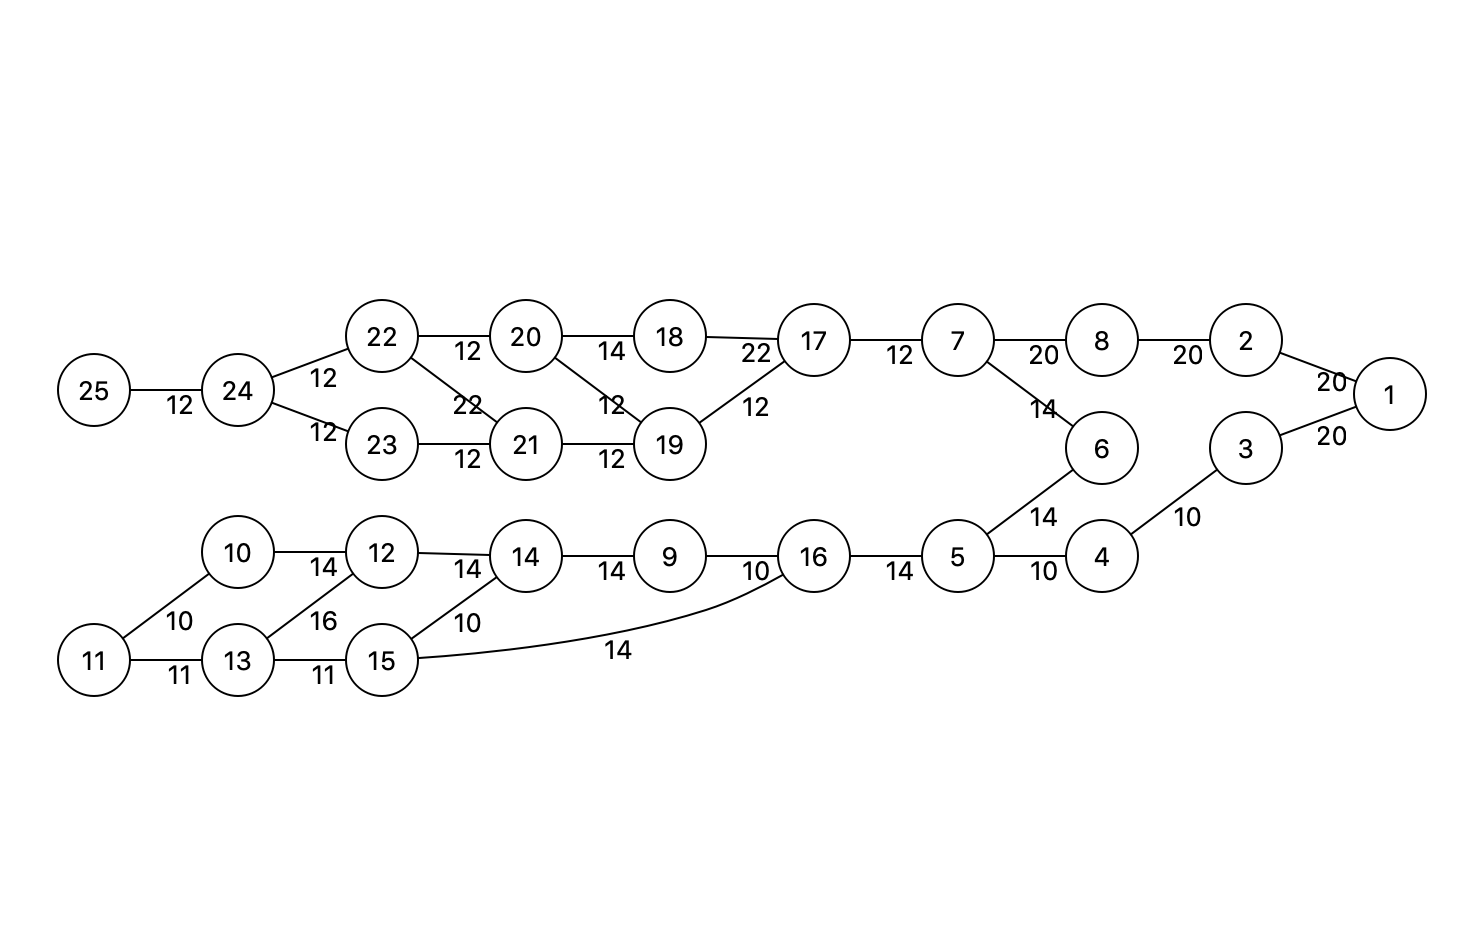
\includegraphics[width=2.7in]{../../Figure/graph_floor_0}} 
		\caption{Ground Floor} 
		\label{fig:subfig_gd} %% label for entire figure 
	\end{figure}
	
	Different floors are connected by those edges denoting stairs and elevators. The representations of all five floors are as follows.  The four exits are labeled $2, 19, 34, 46$.
	\begin{figure}
		\centering
		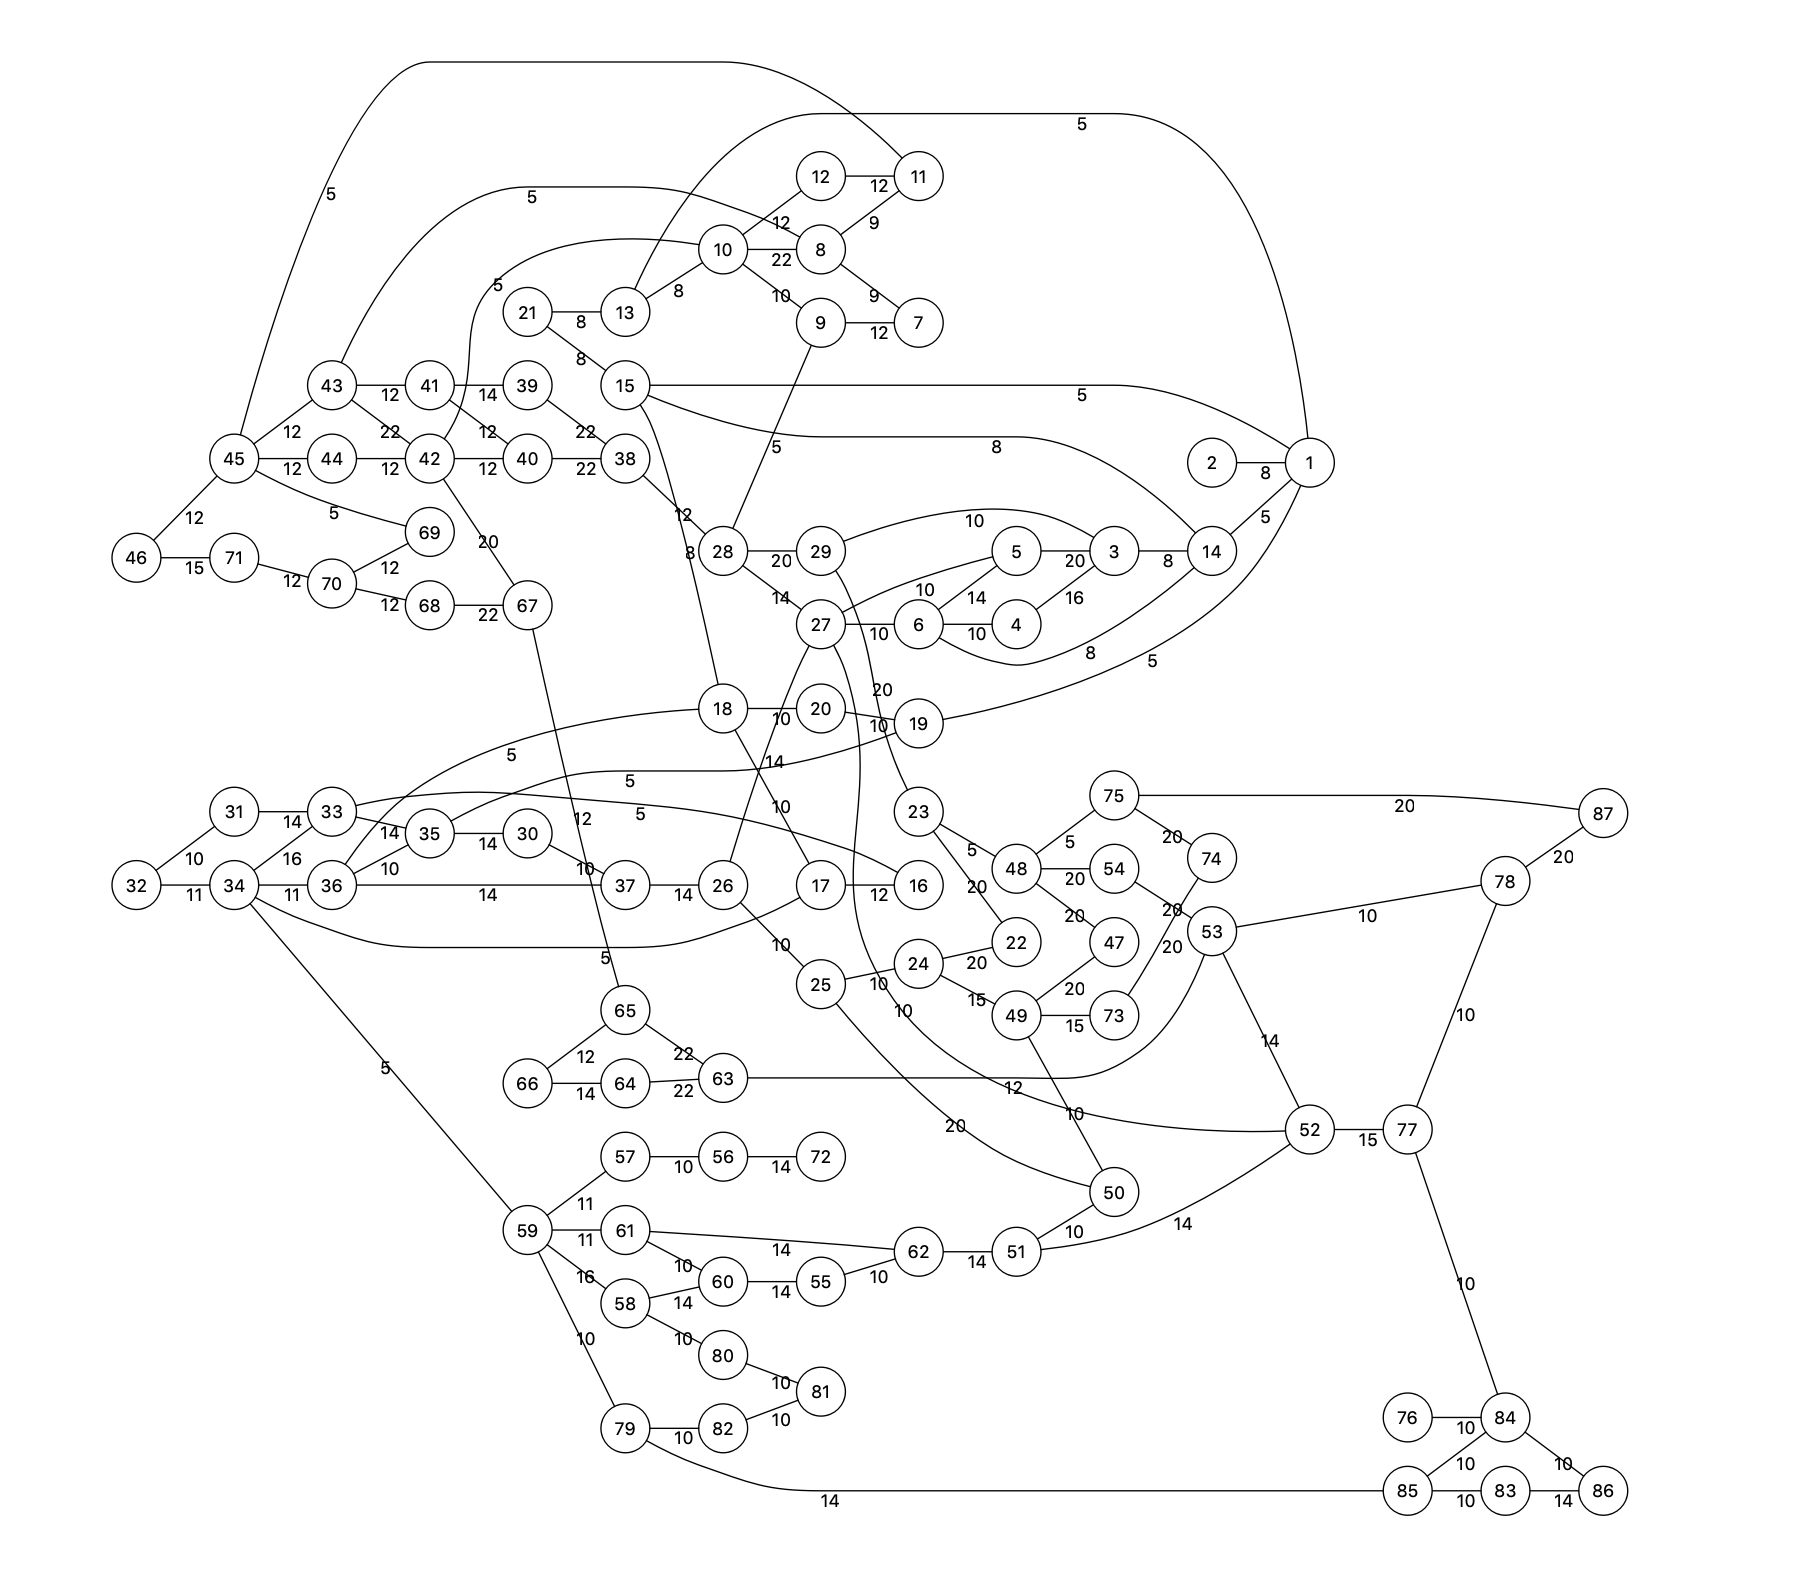
\includegraphics[width=0.8\linewidth]{../../Figure/graph_whole}
		\caption{}
		\label{fig:graphwhole}
	\end{figure}
	
	\subsubsection{Model Description}
	In this model, we assign 26 potential gathering points such as sightseeing sites that initially hold a  number of people. We assume that people  are evenly distributed in these locations. In order to assess the utility payoff of each participant in different initial points choosing specific egress, we introduce the cost $c_R = \sum\limits_{e \in R} c_e$ of choosing this route $R$, where $c_e$ is the cost of choosing an edge on the route. 
	It is reasonable to assume that:
	
	\begin{itemize}
		\item $c_e$ is negatively correlated with the transactional capacity of the edge.
		\item $c_e$ is positively correlated with the length of the edge.
		\item $c_e$ is positively correlated with the number of people on the edge($n_e$),  because the more people choose this route, the more crowded it will be.
	\end{itemize}
	
	In practice, we design the  formula \ref{for_ce} to calcuate $c_e$.
	\begin{equation}
	c_e = \frac{l_e}{v_e}
	\label{for_ce}
	\end{equation}
	,where $vel$ is defined by formula \ref{f_vel}, which model the  connection between the speed of crowd  and the density of the crowd $\rho$ (\ref{for_rho}).
	
	\begin{equation}
	vel=\left\{
	\begin{aligned}
	&1.4 &  \rho \le 0.75 \\
	&1.867 - 0.59 \rho + 0.0412 \rho^2 &  0.75 < \rho \le 4.2 \\
	&\frac{0.42}{\rho} &  \rho > 4.2
	\end{aligned}
	\right .
	\label{f_vel}
	\end{equation}
	
	\begin{equation}
	\rho = \frac{n}{w*l}
	\label{for_rho}
	\end{equation}
	
	In this way, the game plays try to maximize the utility payoff by minimizing the $c$ of the chosen route.
	
	\subsubsection{Model Iteration}
	​       We obtain the average number of people inside the  Louvre to by consulting to the Little's law, and subsequently assign the same numbers of people to each gathering point. The second step is to set a random route preference for each participant as a begin point. Because the change of one person’s choice will also change the velocity of a corridor and thus change the utility payoff of others, this process of iteration is a constantly adjusting process. We continue iterating until no one has a better option – no one has a lower cost of getting out by choosing a different route. At this time, we reach a equilibrium where under a complete rationality assumption everyone ceases to alter their choices.
	
	The model above serves as our preliminary model due to its limitation and next step we will introduce another model to solve the problem comprehensively.
	
	\subsection{Experiment}
	
	\paragraph{Estimated number of people inside the building}
	According to Little's law (formula\ref{for_little}), the long-term average number $L$ of people in a stationary system equals to the long-term average effective arrival rate $\lambda$ multiplied by the average time $W$ that people spend in the system.
	
	\begin{equation}
	{L=\lambda*W}
	\label{for_little}
	\end{equation}
	
	Based on related reports\cite{waittime}, the average people waiting for the Lourve is 3000, which means $\lambda$ is 3000. The average time people spend in visiting is 2 hours. So $L$ is 6000.
	
	
	
	\paragraph{Simulation Results}
	We implemented the game using C++. After 29 iterations, the Nash equilibrium is achieved.  According to the escape route of each escaper at this time, we conducted an escape simulation experiment. We calculate the speed of each person according to the formula \ref{f_vel} and update the location of each person every second. Figure \ref{fig:screenshot001} shows the results, where the abscissa is the escape time interval, and the ordinate is the number of people who escaped within the interval. 
	
	\begin{figure}
		\centering
		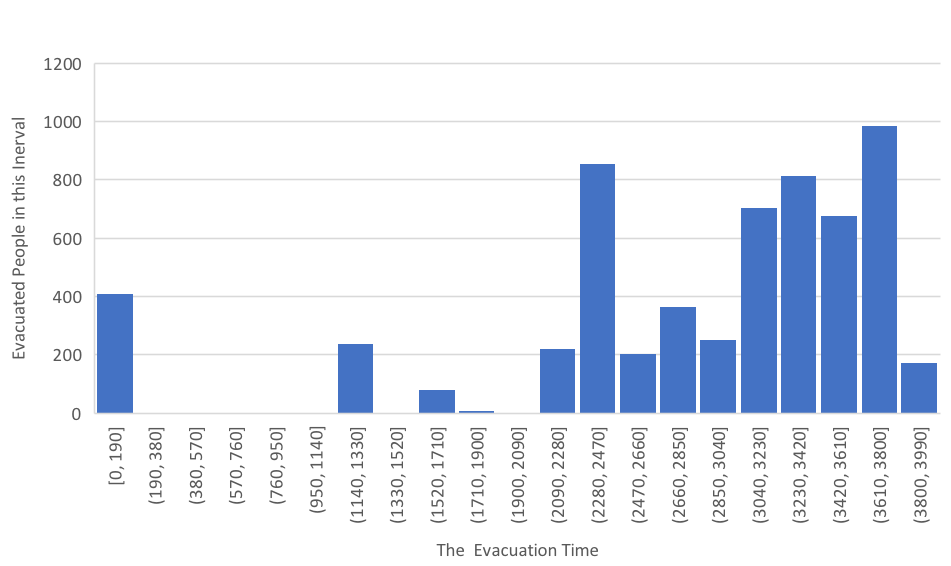
\includegraphics[width=0.7\linewidth]{../../Figure/screenshot001}
		\caption{}
		\label{fig:screenshot001}
	\end{figure}
	
	We found that except for some people of the initial locations at the exit, who escape in no time,  most visitors spent more than 2000 seconds to escape the Louvre. The clearance time is 3812, which is the not an optimistic result when a terrorist attack is go going.
	
	
	\section{Network flow based global optimization model}
	
	
	In the previous game theory model, we determined the best course of action for everyone based on each person's selfish assumptions. However, the evacuation effect is not optimistic. In addition, the model can not be easily modified to address the heterogeneity of evacuees (for example, the existence of disabled people) and the need for emergency people. Therefore, we explored a network flow based global optimization model.
	
	\subsection{Model Analysis}
	
	\subsubsection{Problem transformation}
	
	This model uses a graph to show the architectural construction as the game theory based model. The difference between these two models lies in that the former one use directed edges while the latter one uses undirected edges. We deem each display site in the Louvre as the starting point of evacuation. The problem of evacuating from the four egresses using the shortest time from the starting point can be translated into Minimum-cost flow problem. In order to simplify the model, supersource and supersink are introduced. As shown in figure \ref{fig:screenshot004}, the  supersource $s_{super}$ has an arc with each source node $s_i$,where the capacity of the arc $f_i$ is $s_i$  number of evacuee and the cost $c$ is 0. Meanwhile, there is an arc connecting from sink $ex_i$ to supersink $ex_{super}$. The capacity of the arc is positive infinite while the $c$ is 0.
	
	\begin{figure}
		\centering
		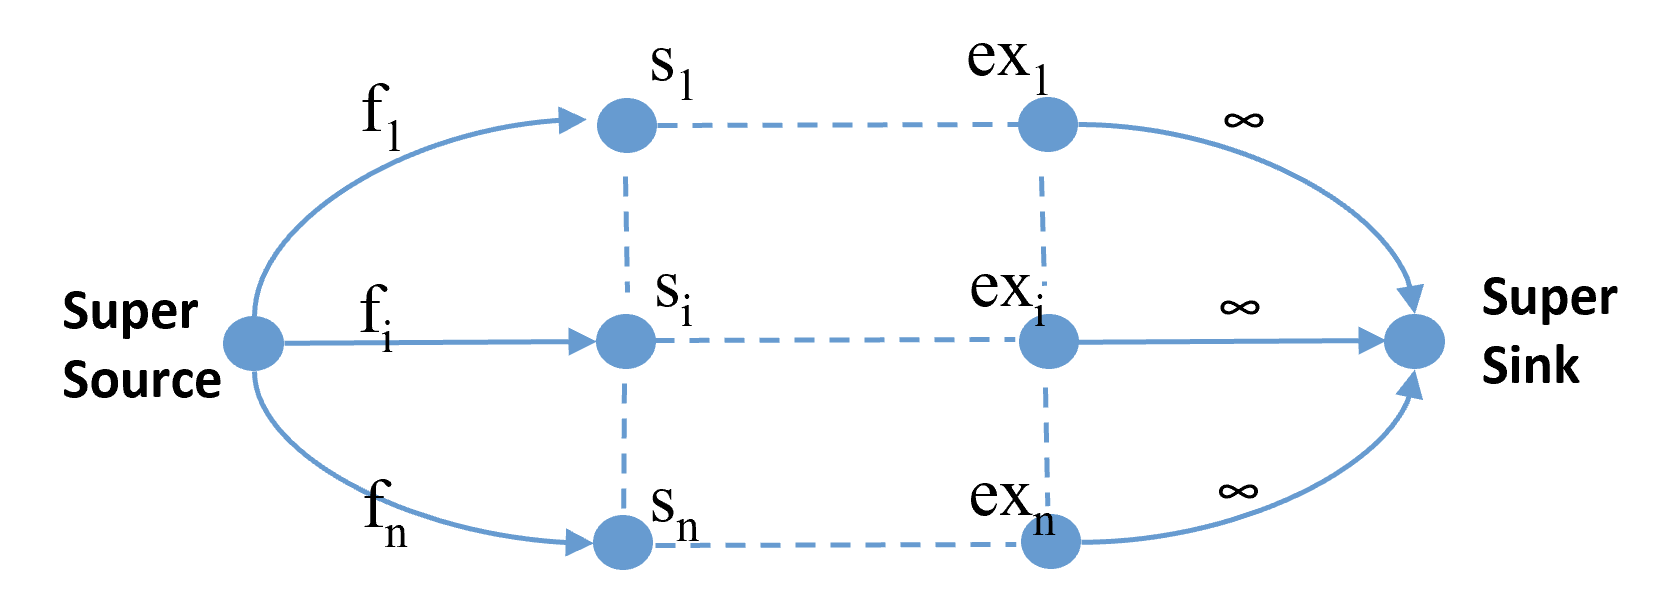
\includegraphics[width=0.7\linewidth]{../../Figure/screenshot004}
		\caption{}
		\label{fig:screenshot004}
	\end{figure}
	
	\subsubsection{Charactersitics of arcs capacity}
	
	\paragraph{The instant flow capacity }
	Given a certain arc with width $w$, we set the  formula of instant flow capacity based on two variables, which are  rate and density: $f=vel * \rho$.  Among the formula, $vel$ represents people's walking rate and $\rho$ represents the crowd density,as defined by formula \ref{f_vel} and \ref{for_rho}. Flow capacity represents the number of people going through a cross-section within a certain time.
	
	\paragraph{Maximum flow in the arc }
	
	Take max$f=v_m\rho_m$ as the maximum flow of the channel. This flow is commonly referred to as a saturated stream. In the formula, $v_m$, $\rho_m$ are called critical speed and critical density, respectively.If the value is the upper limit of the capacity of the arc $a(v_i,v_j)$, the lower limit of the capacity is the maximum number of people passing through the channel when the channel is blocked. The max is calculated by interpolation of Equations 1 and 2, resulting as when the crowd density is 2.00 persons/m2 and at a speed of 0.85 m/s, the $f​$value is the largest.
	
	\paragraph{Accumulative flow}
	During a certain time period$t$, we define the total flow passing through an arc as 
	$$
	F = \int _{0}^{t} f \Delta t = t * f
	$$
	
	\subsection{Experiment}
	
	As well, we have used C++ to construct this model. By utilizing iteration, we gradually add up the evacuation time $t$, until the total amount of evacuated people during $t$ have reached 6000, as we have estimated in the former model. We set the starting point equal to what we have done in the previous model.
	The result of the experiment reveals that it is possible for 6000 people to evacuate successfully in 647 seconds.
	
	\subsection{Improvements}
	
	\subsubsection{Coordinate efficiency and safety}
	We assume that the crowd travels with the highest density together with the corresponding speed, as we have discussed previously. However, it is not feasible to guarantee each individual travel in this condition. Hence, we introduce a "tradeoff" factor, $\alpha$, into the model aiming at efficiency and safety. As a result, we modify the formula into
	$f=\alpha * vel * \rho$. 
	
	We take a value every 0.01 within interval [0.5,1.0], trying to achieve the optimal evacuation time under every $\alpha$. The results are shown in figure \ref{fig:screenshot002}. It is shown that the absolute value of the gradient of the curve increases while $\alpha$ goes down. In conclusion, it is an efficient "tradeoff" way to set the value of $\alpha$ between 0.8 and 0.9.
	
	\begin{figure} 
		\centering 
		\subfloat[Evauation time under different $\alpha$]{ 
			\label{fig:screenshot002} %% label for first subfigure 
			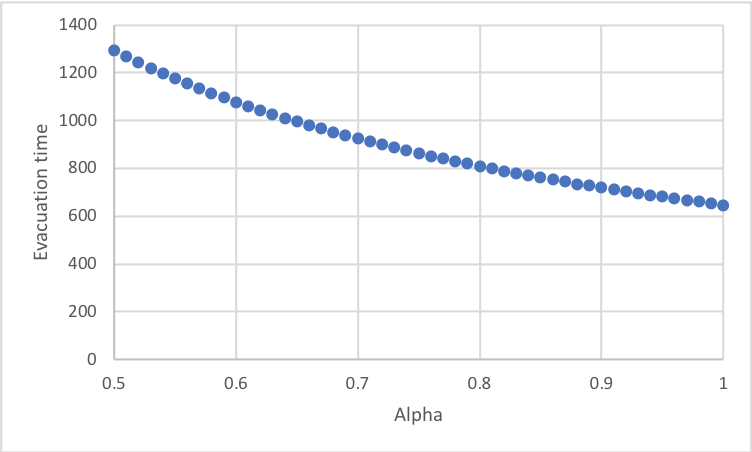
\includegraphics[width=2.7in]{../../Figure/screenshot002}} 
		\hspace{0.2in} 
		\subfloat[Parallel edges]{ 
			\label{fig:screenshot003} %% label for second subfigure 
			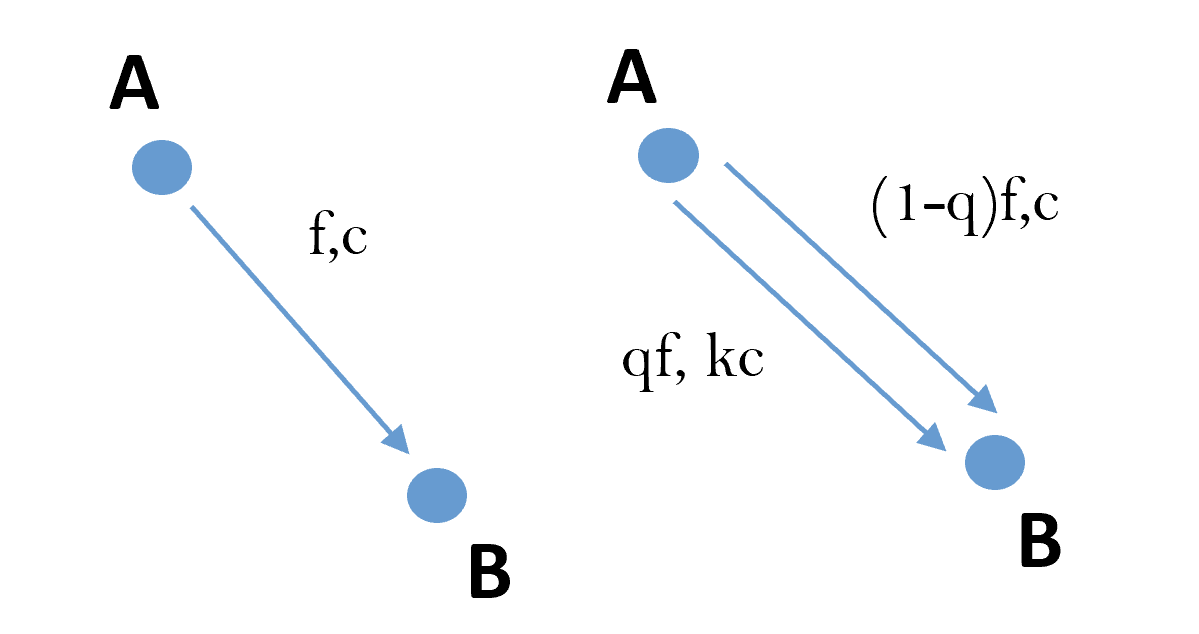
\includegraphics[width=2.7in]{../../Figure/screenshot003}} 
	\end{figure}
	
	\subsubsection{Evacuations path for people with restricted mobility}
	
	Our model aims to serve not only the sound people  but also the elders and disabled individuals. Since those visitors have restricted mobility, we take this type of visitors into consideration and achieve a result. We introduce parallel arcs. Assuming that the disabled take up a proportion of $q\%$, then those imported parallel arcs will take over $q\%$ flow of the original arcs whose cost is $k$ fold of the original one.
	During the experiment, we set $q$ as 0.1, $k$ as 2. According to the result, the total cost of evacuation only improves by $2.6\%$.
	
	\subsubsection{Arrival for emergency personnel}
	When terrorists enter the Louvre to launch the attack, it is necessary to not only evacuate visitors but also sending emergency people to operate rescue work.  As long as there are many people trying to get into the building while visitors all trying to get out, convection happens. Our model introduces reversed edges to address convection. In the bi-directional network, reversed edges are arcs sharing the capacity with the arc with an opposite direction. Denoting the capacities of the original arc and the derived forward arc and reversed arc as $f$, $f_A$, $f_B$, then it satisfies $f = f_A + f_B$. As is shown in the chart \ref{fig:screenshot005}, we introduce a virtual point, C, reverse the difficult problem about the flow quantity of two reverse edges, into the flow capacity $f$ going through $C$. Furthermore, we divide the virtual node into two parts, $C_{+}, C_{-}$. As the figure \ref{fig:screenshot006} has shown, we can transform the problem into controlling the flow between $C_{+}$ and $C_{-}$, which is a question based on trivial network flow. In this way, our problem gets done.
	
	
	\begin{figure} 
		\centering 
		\subfloat[]{ 
			\label{fig:screenshot005} %% label for first subfigure 
			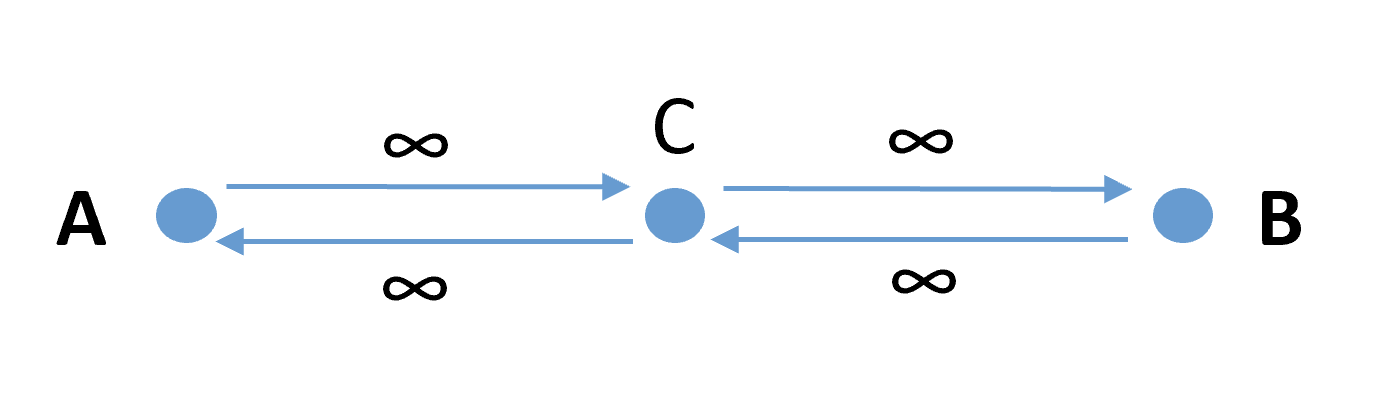
\includegraphics[width=2.7in]{../../Figure/screenshot005}} 
		\hspace{0.2in} 
		\subfloat[]{ 
			\label{fig:screenshot006} %% label for second subfigure 
			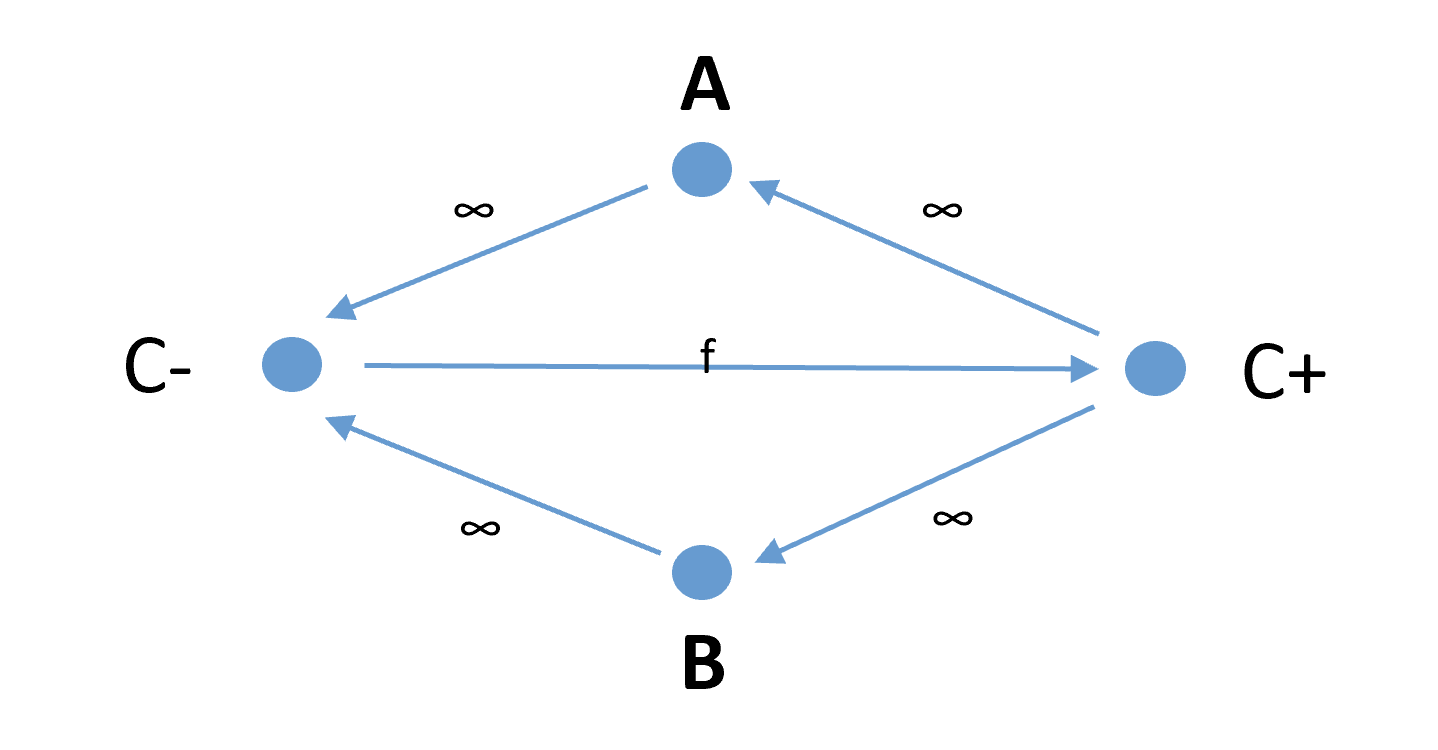
\includegraphics[width=2.7in]{../../Figure/screenshot006}} 
	\end{figure}
	\subsection{Bottlenecks}
	In previously works, network flow has been employed to analysis the evacuation bottlenecks. The network flow transshipment algorithm \cite{white1972dynamic} used in EVACNET+ and SAFE-R considers the bottleneck in evacuation is on the passageway or staircase while the fast flow control algorithm \cite{chen2009fast} assumes that doors would be the bottleneck in most evacuation cases because the widths of passageways and staircases are wider than egress doors. 
	
	In our model, we determine the bottleneck in the building by examining the flow from the source nodes given certain evacuation time. At the same time, the source of the smallest flow will evacuate visitors at the lowest speed.
	The result of the experiment says that visitors at the hall located in the upper left and the bottom right corners of the first floor evacuate in the last minute, as marked by the red box in figure \ref{fig:screenshot007}. According to the iconography, there is no stair or elevator close to these two corners, the path of which is narrow as well. This phenomenon should arise enough attention and modification.
	
	\begin{figure}
		\centering
		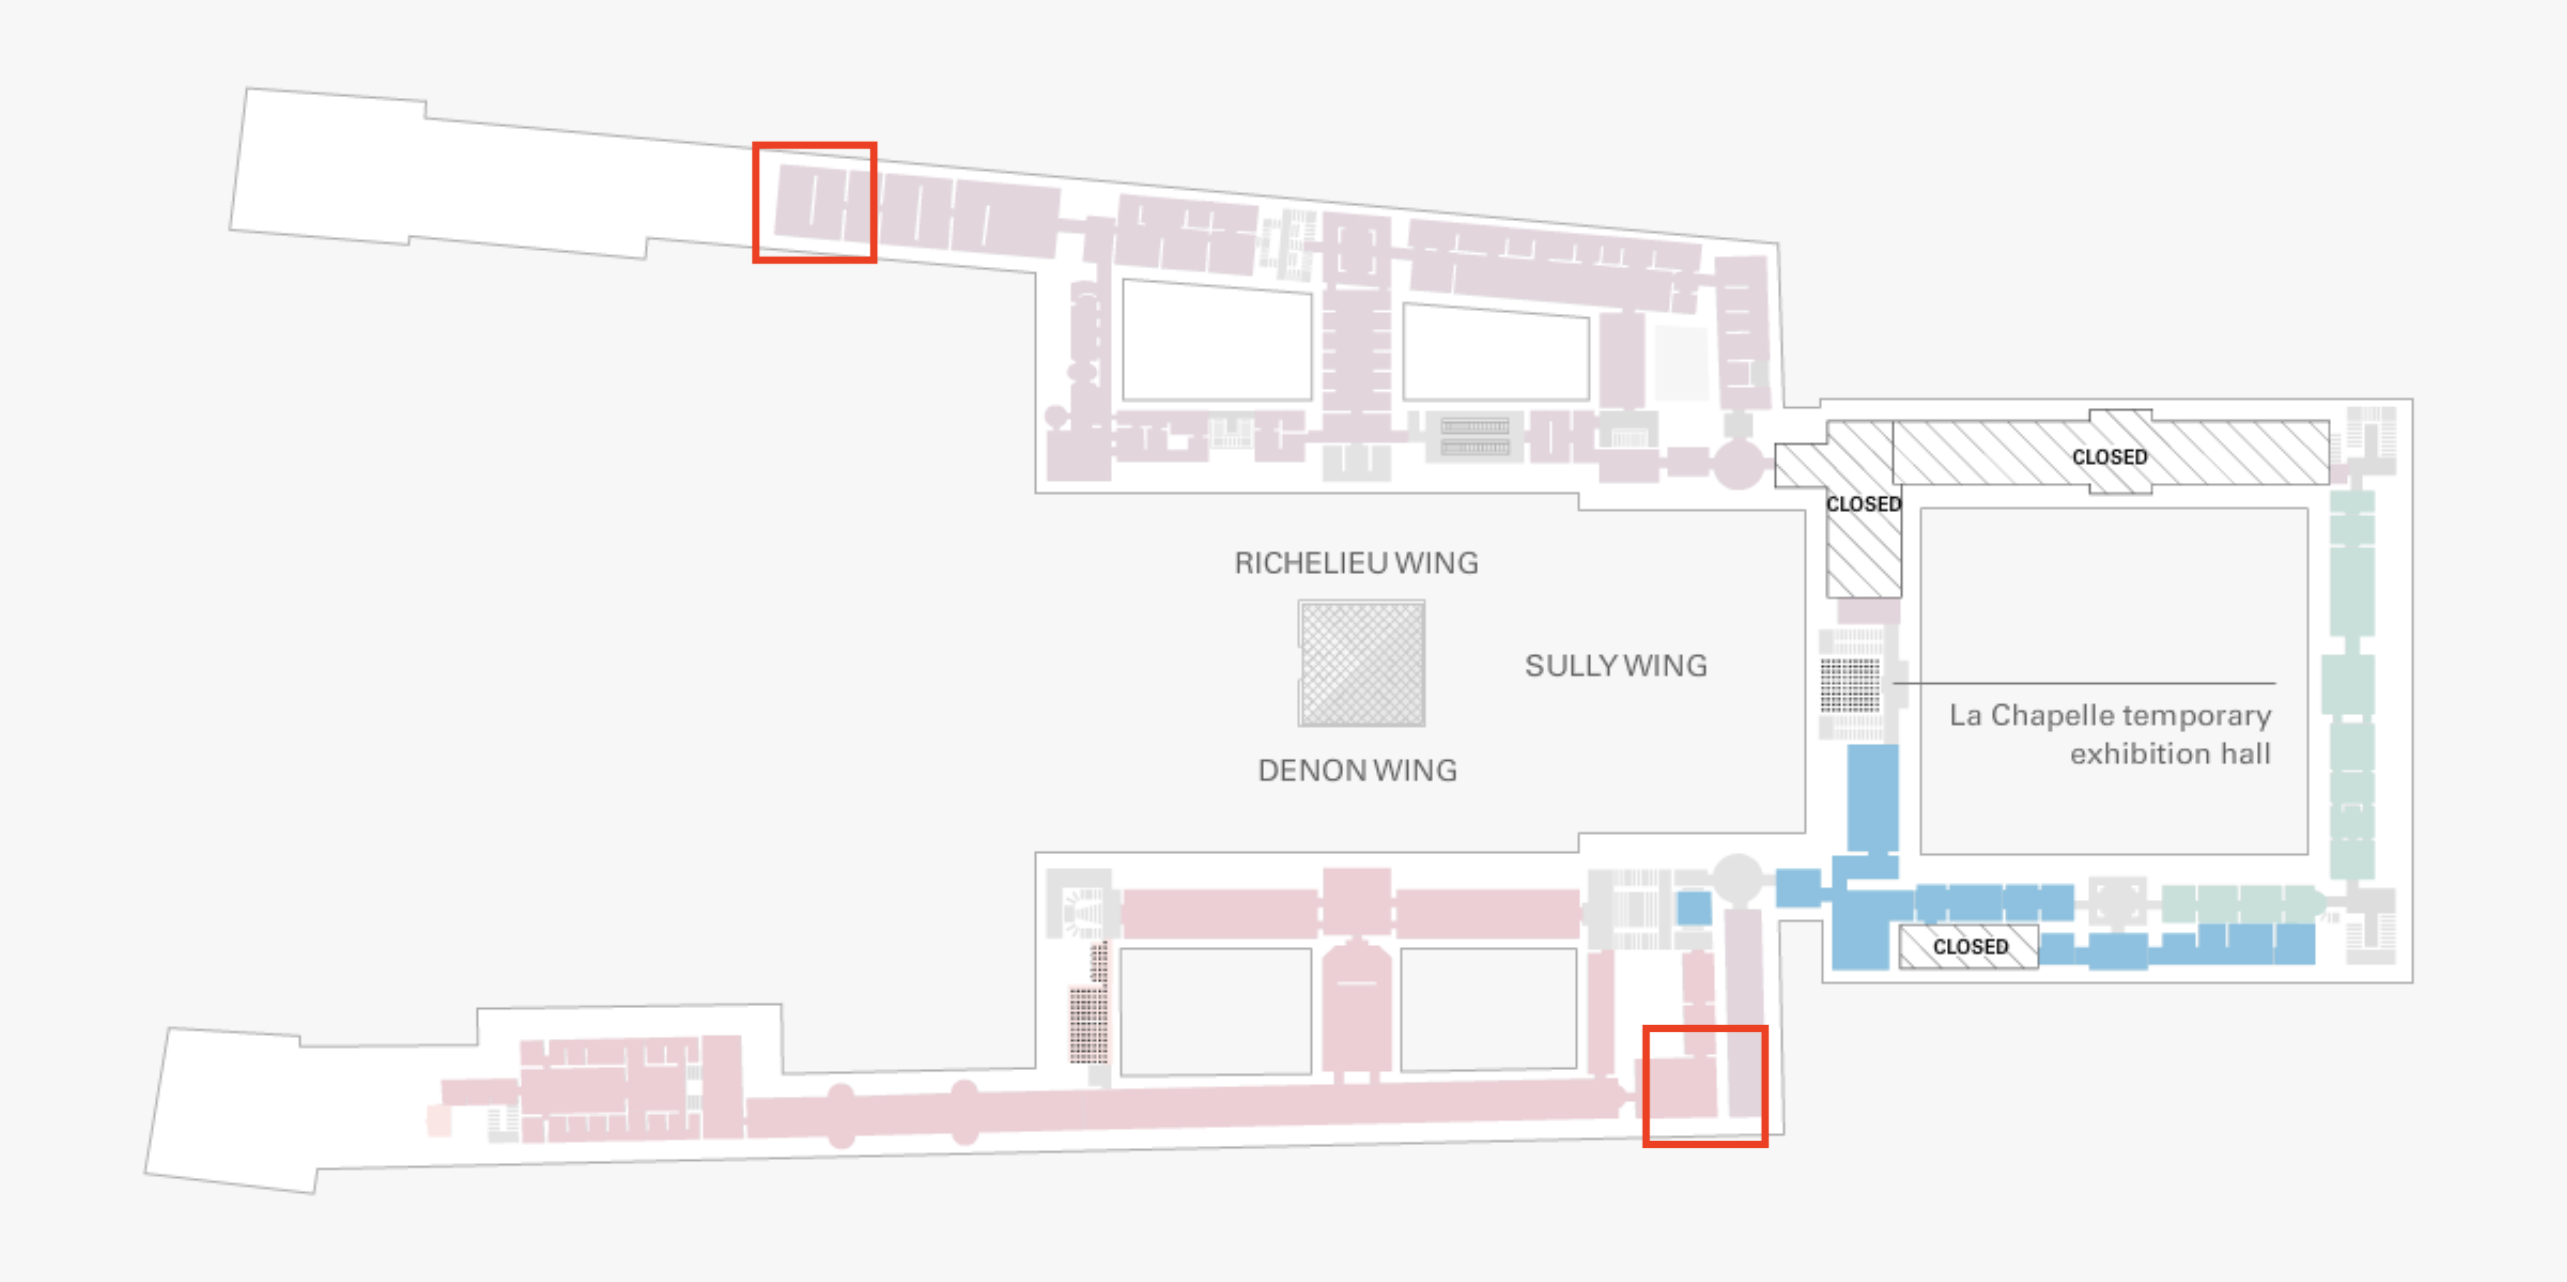
\includegraphics[width=0.7\linewidth]{../../Figure/screenshot007}
		\caption{Ichnography of 1 floor}
		\label{fig:screenshot007}
	\end{figure}
	
	
	\section{Technical Facilitation}
	
	\subsection{App, such as "Affluences"}
	As the figure below, "Affluences" provides information at every main entrance, especially how many people are waiting at the entrance for admission.  This can be used to analyze which entrance is more suitable for evacuation, instead of stimulating a larger scale of fear in the crowd. Using the entrance with fewer people waiting for admission can enhance the moving speed of the crowd when rushing out of the entrance into a safe area.
	Meanwhile, it is feasible to insert a warning system in the application. This system can trigger the alarm on every smartphone when it receives the evacuation signal. More remarkably, this alarm should be broadcast in different languages, depending on the system language every visitors choose to apply to their phones. In this way, the "Afflunces" is able to call for instant attention on the evacuation instruction when terror attacks happen.
	
	\subsection{Autonomous Navigation System using Mobile Phones}
	
	There are two difficult problems pertain to the selection of an evacuation route according to each individual's situation, especially their location and environment. Using technology to define two essential information. First is the constant supervision of the situation of living space and the detection of dangerous situations. Second is the detection of residents' respective positions.
	
	There are existing technologies using the cell phone or PDA for indoor navigation. The wireless beacon signals are especially used for this function. The user's device receives wireless beacon signals from the surrounding environment and can thereby detect a user's position by a mobile terminal independently. This system is capable of performing robust positioning in noisy environments. Meanwhile, it provides autonomous positioning in the cell phone as long as reliable performance in crowded environments. All these advanced functions assure the emergency evacuation can be operated efficiently and correctly, In this way, visitors can be evacuated out of the Louvre fast and safely.
	
	Specifically speaking, this technology provides the Louvre management with several inspirations. First of all, utilizing the sensor-data management system to manage the information needed for evacuation in real-time mode. Secondly, installing various sensors in the Louvre to detect emergencies and integrate the situation in time. Last but not least, the wireless beacon devices in the environment can navigate people correctly when evacuating. Meanwhile, it involves no stationary terminal, but portable terminals.
	
	It is obvious that using this kind of indoor emergency evacuation service can effectively improve the feasibility of the evacuation plan.
	
	\section{ Utilizing other entrances}
	
	\subsection{Entrance for the emergency personnel}
	Since emergency personnel such as firefighters, doctors and SWAT, are essential for managing situations after terror attacks. In this way, as terror attacks happen, it is necessary for emergency personnel to get to the scene immediately. 
	
	Meanwhile, visitors' evacuation routes should be taken into consideration. The arriving of emergency personnel cannot obstruct the evacuation path. 
	
	Hence, it is proper to open other entrances for emergency personnel to get into the museum. Together with the discussion of merit and demerit of opening other entrances to the public, an appropriate solution will be presented later.
	
	\subsection{Egress for the visitors}
	
	As the problem states, there are others available exits only known to the staff. It is obvious that opening these entrances will make changes to the evacuation plan. We are going to list the benefits and shortages of utilizing these entrances as additional evacuation path.
	
	\subsubsection{Benefits}
	
	Apparently, opening more exits to the public helps increase the efficiency of evacuation. Precisely, more possible ways for evacuation arrangement, more quickly the visitors can be instructed out of the Louvre.  The improvement of efficiency can be viewed from two aspects.
	
	a. It can help alleviate the burden of evacuation at those famous exhibition halls. For example, the hall displaying Mona Lisa is crowded with people all year round. If opening nearby entrances for visitors to evacuate, there will be a smaller flow of people rushing out of the main four entrances. In other words, available extra exits benefit the most crowded halls to great extent.
	
	b. In less crowded places, more available exits help to instruct people to various paths, which will not aggravate the most crowded entrances. Flows from different rooms can avoid colliding with each other since there are more entrances for people to evacuate.
	
	\subsubsection{Shortages}
	
	However, there are still abundant shortages when opening more exits to the public. Shortages are listed below, considering maintaining cost, security and other messy results.
	
	a. maintaining cost
	
	As it states in the Problem, those available doors are only known to the staff. Some of which are employee entrances and old secret entrances built by the monarchy. It can be implied that these doors are not suitable for large amounts of visitors to rush out in their original conditions. Hence, maintaining or repairing those available exits cost much budget.
	
	b. lack of security
	
	To secure the precious cultural relic in the museum, the security at the main entrances must be rigor, using various advanced techniques to eliminate the danger. However, other doors are not used for regular entry, with no sufficient security. It provides the possibility for criminals to enter the building when disorders take place.If less-secured exits are open to the public, it is definitely that the Louvre will suffer from more risks.
	
	c. messy situations
	
	If opening more exits to the public, there must be certain people being directed to those exits. When they notice that most people are rushing to the main entrances, hesitation and disobedience towards the instruction appear. As a result, this will lead to messy situations, such as collision with each other.
	
	From this aspect, opening more exits do no good to the evacuation instruction.
	
	d. infeasible to open those entrances immediately as soon as emergency happens
	
	It is not feasible to open all those entrances immediately as soon as emergency happens. Because it also takes time for the staff to get to the specific entrances, which is not practical while evacuating.
	
	\subsection{Appropriate Solution}
	
	Since opening exits in addition to the four main entrances has both advantages and disadvantages, it is necessary to discuss the appropriate solution for utilizing those exits. The solution consists of two aspects, when to use and how to use, as described below.
	
	\subsubsection{When to use}
	
	Mainly considering the shortages those exits cause, we recommend using the exits only for emergency take place. At regular times, those exits are closed for fundamental security.
	
	However, when potential threats such as fire or the attack scenes block out some segments of evacuation path, the alternate exits should be open for evacuation. Meanwhile, it should be noticed that the utilization of the additional exits should match with the level of the emergency since the safety factor of each kind of doors differs. Specifically, VIP entrances are of high safety factor which is suitable to act as an evacuation exit. Nevertheless, secret entrances built by monarchy are of extremely low safety factors, which means if there is no extra-severe attack happens, these secret entrances shouldn't be open.
	
	\subsubsection{How to use}
	
	In terms of the number of exits can highly improve the efficiency of the evacuation plan near the famous exhibition halls, the Louvre can utilize those entrances. For example, the hall displaying the Mona Lisa or the second floor of the Denon Wing.
	
	Meanwhile, we recommend a daily maintaining procedure to ensure the safety of those paths.
	
	As for the possible messy outcoming, it is feasible to emphasize that the instruction is the optimal solution for every individual. Only in this way can make sure that the crowd follows evacuation guidance.
	
	\section{Sensibility}
	
	When a terror attack happens, it is likely that a power failure takes place at the same time. As a result, elevators get out of order, leading to altering the architectural construction. Therefore, the available flow capacity decreases. We testify whether our model can function properly under this condition. Eventually, our shortest evacuation time increase from 647 seconds to 1035, which is 59.9\% of the original time, showing a significant impact.
	
	Take another case as an example,  terrorists may launch an attack at any time when daily routine works such as refurbishment and porting are carried out, which blocks access to part of the aisles. By cutting all the pass one by one, we find out that cutting the aisle between lift P on the first floor and Passage Richelieu entrance is of vital significance to overall evacuation time. It will add to the evacuation cost by 247687 compared to the previous cost of 1640757.
	
	\section {Scalibility}
	The Louvre is the largest museum building in the world. Our two models' successful application is a good demonstration of their scalabilities. However, if we want to perform a more accurate analysis of the evacuation path, we should model the Louvre using Graph $G$ with more nodes and edges. In addition, consideration should be given to the situation during the peak passenger flow period.  It must be tested whether the model is still valid when increasing the number of registered visitors.
	
	We first carry out theoretical analysis,  the DFS algorithm with cycle detection is used in the model based on game theory. Considering the number of nodes, the DFS algorithm has exponential time complexity and is not scalable. Therefore, in practice, we use the depth-limited DFS algorithm. In this way, a part of the  evacuation routes can be found in a limited time, which is in line with the model needs.
	Theoretically, the dynamic game process will reach the Nash equilibrium. However, when setting different numbers of people in the building, the number of iterations required to achieve equilibrium is unpredictable. Therefore, we conducted numerical experiments and obtained the number of iteration till convergence for the cases where 6000, 10000, 15000, 20000, and 30000 are in the museum. Results are shown in figure \ref{fig:screenshot008}.
	
	\begin{figure}
		\centering
		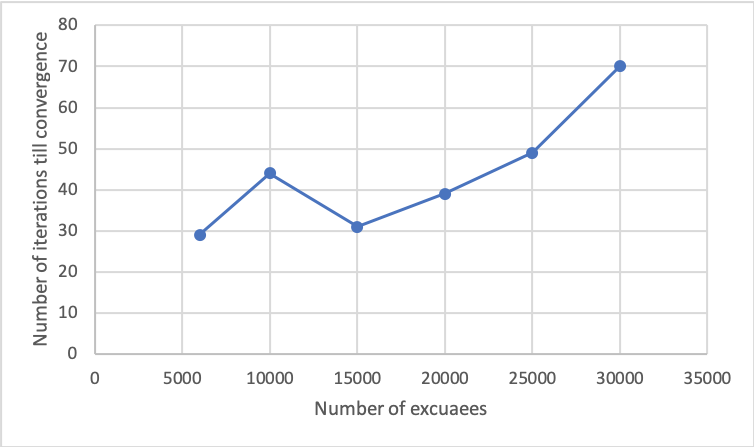
\includegraphics[width=0.7\linewidth]{../../Figure/screenshot008}
		\caption{}
		\label{fig:screenshot008}
	\end{figure}
	Although it can be seen that the number of iterations has an exponential growth trend, a passenger flow that is more than five times higher than  usual has been difficult to appear. Therefore, the model remains scalable within the scope of the given problem.
	
	As for the network flow model, it is essentially a polynomial time solution to the linear programming problem. Even if the number of nodes is extended by 10 times, the result can  run in a short time, which is a very scalable method.
	\section{Model evaluation}
	\subsection{Evaluation on the game theory based model}
	\paragraph{Strengths}
	
	\begin{itemize}
		\item  For this model, there are two obvious strengths that we insist. Firstly, this model is based on  behavior simulation of discrete objects and use authentic data to an achieve relatively reliable simulation outcome. 
		\item The Nash Equilibrium allows individuals to attain the optimum choice on their own. Due to selfishness, it is feasible for people to accept the calculated results.
	\end{itemize}
	
	\paragraph{Weakness}
	\begin{itemize}
		\item It should also be noticed that, there are few problems with this model. First of all, this model assumes that everybody is totally aware of the others' choices. However, in the actual scenes of evacuation, an individual is only aware of nearby ones' evacuation choice. Moreover, people are impossible to realize every evacuation path. 
		\item Additionally, even though this model gives an optimal choice for every individual, it will by no mean affect overall evacuation speed. In this way, this model is not suitable for instructing people getting out of the Louvre safely and efficiently. In other words, some people will be left behind with an extremely long evacuation time.
	\end{itemize}
	
	\subsection{Evaluation on the optimized evacuation time model}
	\paragraph{Strengths}
	
	\begin{itemize}
		\item The optimized evacuation time model based on network flow, aims to develop the optimum solution for the whole situation. Taking the previous model as comparison.
		\item The optimized evacuation time model has great scalability, which can be applied to complex situations under various restrictions. It can perfectly fit in with the restrictions given by the problem, providing reasonable path for disabled people and foreign visitors.
	\end{itemize}
	
	\paragraph{Weakness}
	\begin{itemize}
		\item The transparent weakness of this model is that, it assumes each individual definitely obey any command. However, it is unrealistic in the application, since people all tend to speculative choices.
		
	\end{itemize}
	
	\section{Future work}
	
	To sum up, we design two models to solve the problem from two different perspectives and the results are distinct. Both models have their limitations in terms of applicability such as the maximum evacuation time for the last person is very long. So we have to do a lot more to improve our work.
	Firstly, the game theory based model and the network flow based model reveal different outcomes, among which one is best for every individual while the other is best for the whole situation. It is more applicable if we can generate these two models together to create a solution to satisfy everyone individually and wholly.
	Secondly, we did not consider the interacting behavior of the crowds and the familiarity of the building as important factors in evacuation. Future work may include  factors like these.
	\newpage
	Dear sir,
	
	Upon hearing that the executive of the Lourve is working on formulating policy and procedure to upgrade emergency management of the Lourve aiming dealing with the non-traditional emergency, my fellow colleagues and I are honored to engage in clearly communicating our role and scope of engagement in the development of emergency evacuation plans. We have been working with painstaking efforts so as to do something for the Lourve concerning precaution of terrorist attacks, and we do have some results by researching day and night these days. We truly hope that we can be of help in providing proposed crowd management recommendations and emergency evacuation procedures for the Lourve to ensure the safety of visitors and the staff.
	
	Inspired by optimization model, we established a smart evacuation model based on network flow that allows visitors to leave the Lourve as quickly and safely as possible. Based on the results of our models, we recommend some feasible policies both on emergency evacuation and the crowd management for your reference.
	
	The policy strategy for emergency evacuation should be based on the risk evaluation of the surrounding environment. Immediate upgrade for emergency plans are necessary on the grounds of that miscellaneous threats will emerge in various ways. Furthermore, safety measures for organizational and architectural construction and digital monitor shall be in balance. The Lourve ought to mark the emergency exits noticeably and reconstruct the ‘secret exits’ for emergency use. Emergency shelters for special people such as the disabled should be taken into consideration due to their restricted mobility. Above all, the staff and emergency personnel are required to execute adaptable plans to respond in an emergency.
	
	In terms of crowd management,  particularly indoor space evacuation, it is necessary to pay attention to the total number of people before the start of evacuation and to properly control the rationalization of the size of the population entering the system. According to game theory, individual always seeks the optimum solution for itself, in other words, the crowd will choose the way that is advantageous to them. Nevertheless, to evacuate efficiently as a whole, one may sacrifice his optimum solution but adhere to the overall optimum solution. As a result, we firmly believe that ground personnel ought to receive professional train to maintain order and control the crowd.
	
	As mentioned previously, the scalability of evacuation time optimization model based on network flow illustrates that the model can be modified and adapted to applications for other large, crowded structures. It is highly recommended that the Lourve keeps liaison and coordination with other museums or buildings in order to exchange experience on emergency evacuation plans. 
	
	Finally, we sincerely suggest that emergency drills are held regularly according to the estimated time and routines for emergency evacuation based on our evacuation time optimization model.
	Best regards,
	
	The ICM team
	
	
	\section{Reference}
	\bibliographystyle{IEEEtran}
	\bibliography{final}
	
\end{document}
